\subsection{Maximale Leistung bei variabler Spannung}\label{subsec:LeistungSpannungsabfall}
In diesem Versuch wird die maximale Leistung bei einem Spannungsabfall untersucht. Da die asynchrone Maschine nicht für 3800 RPM ausgelegt ist, wurde dieser Versuch bei einer konstanten Drehzahl von 3600 RPM gemessen. Wie im vorhergehenden Versuch, wurde das Drehmoment aufs Maximum eingestellt, während die Spannung langsam erhöht wurde.


\begin{figure}[H]
	\centering
	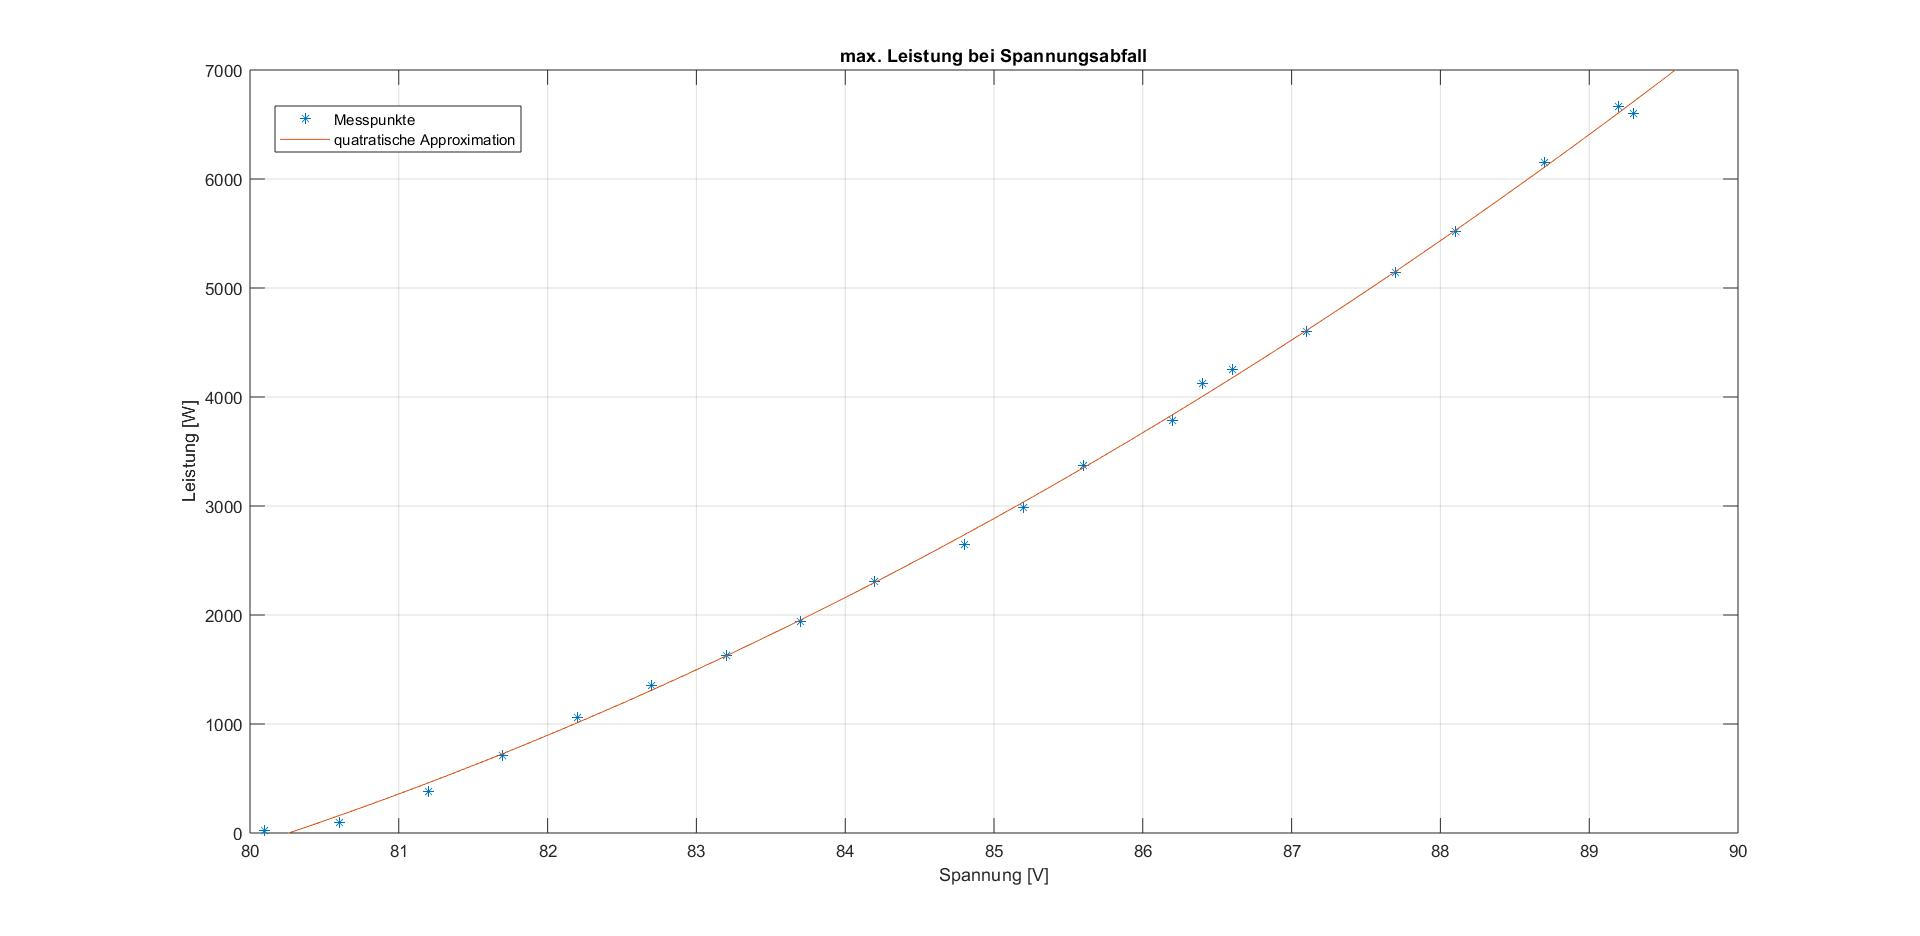
\includegraphics[width=0.8\linewidth]{maxLeistung.jpg}
	\caption{Maximale Leistung}\label{fig:maxLeistung}
\end{figure}

Unter der Annahme, dass zwischen der maximalen Leistung und der Spannung ein quadratischer Zusammenhang besteht (rote Approximation), ist anzunehmen, dass die maximale Leistung bei 3600 RPM und Nennspannung (96V) bei 15kW liegt. Hierbei ist jedoch anzumerken, dass die effektive Leistung an der Welle des BLDC-Motors ca. 10\% höher ist, da diese auf der elektrischen Seite der asynchronen Maschine gemessen wurde.
 